\chapter{Estado del arte\label{cap:estadoDelArte}}

En este capítulo se presenta la única plataforma de captura y reproducción de tráfico de red que se basa en la misma \gls{FPGA} que este Trabajo de Fin de Grado, \textit{The Open Source Network Tester}.
Adicionalmente, se exponen también (brevemente) otras herramientas similares de captura, reproducción y análisis.
Se intenta por tanto detallar de forma objetiva los aspectos positivos y las carencias de las distintas alternativas, poniendo así en contexto el proyecto a desarrollar.
Dado que la naturaleza de este proyecto es desarrollar una interfaz web, se hace especial hincapié en la interfaz de usuario de la que dispone cada uno de los sistemas analizados.

\section{The Open Source Network Tester\label{sec:eda:osnt}}

\textit{The Open Source Network Tester (OSNT)}~\cite{osnt} es un generador y capturador de tráfico.
Esta aplicación se ejecuta sobre cuatro \textit{NetFPGA-10G} (que como ya se ha comentado, es el mismo modelo de sonda que el seleccionado en este proyecto).
\textit{OSNT} permite generar o capturar paquetes de todo tipo de tamaño, y establecer la tasa a la que se realizan estas operaciones.

Una de los puntos fuertes de \textit{OSNT} es que tanto el diseño \textit{hardware} como el \textit{software} son de código abierto, y pueden ser modificados.
Se facilita así extender la aplicación para soportar nuevos protocolos.
Otra característica relevante es que posee una interfaz gráfica de usuario desde la que manejar la sonda de red (ver Figura~\ref{fig:osnt}).
Esta interfaz permite configurar la captura o reproducción seleccionando la velocidad de transmisión.

Sin embargo, se han detectado también algunas carencias y aspectos susceptibles de mejora en \textit{OSNT}.
En primer lugar, no gestiona algunos elementos que están relacionados con la sonda y que podría ser de utilidad.
Por ejemplo, no controla que el sistema de archivos tenga una velocidad de escritura suficiente para la captura, lo que puede afectar al rendimiento y hacer que no se aproveche al máximo la sonda de red.
Tampoco comprueba que el espacio disponible dentro del disco sea suficiente antes de programar una captura.
Por último, no permite una gestión activa de las \glspl{traza} almacenadas (clasificación, detalles, borrado de las mismas, etc.).

Respecto a la interfaz, se han identificado algunas áreas que podrían ser perfeccionadas.
Una de ellas es que no es posible conocer el estado de la sonda de manera intuitiva, y tampoco existe una clara separación entre captura/reproducción y módulos adicionales.
Asimismo, gran parte de la información que se muestra en la interfaz podría ser agrupada en forma de gráficos, visualmente más atractivos.
Se echa de menos además soporte para varios idiomas, algo que facilitaría la utilización de la aplicación a usuarios no angloparlantes.
En términos de arquitectura, el sistema requiere de acceso físico (o remoto por \textit{ssh}) al servidor para su manejo, cuando podría ser útil exponer la funcionalidad como un servicio accesible desde cualquier dispositivo.
Para terminar, el hecho de que la interfaz esté sobre el propio servidor de la sonda tiene como consecuencia que si el sistema se saturase, la interfaz podría quedar inutilizable.

\begin{figure}[H]
  \centering
  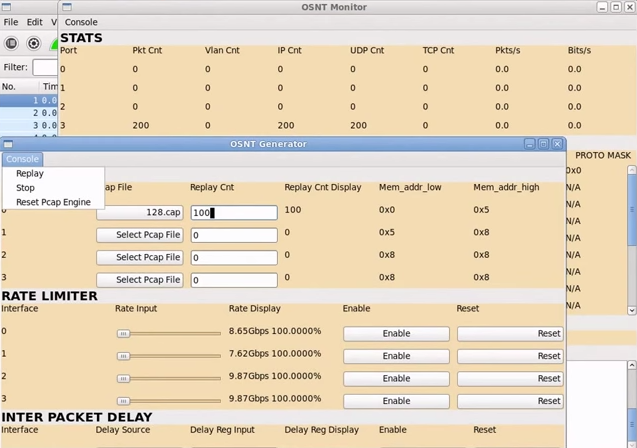
\includegraphics[width=\textwidth,clip=true]{graphics/capturas/osnt}
  \caption{Captura de la interfaz gráfica de \textit{OSNT}.}
  \label{fig:osnt}
\end{figure}

\section{Otras herramientas similares\label{sec:eda:otras}}

\subsection*{tcpdump y libpcap\label{sec:eda:tcpdump}}

La utilidades \textit{tcpdump} y \textit{libpcap}~\cite{tcpdump}, implementadas como librerías, permiten analizar el tráfico que circula por la red.
Así, el usuario puede capturar y mostrar en tiempo real los paquetes transmitidos y recibidos en una red a la que el ordenador esté conectado.
Se suele utilizar para depurar aplicaciones que envían y reciben tráfico de red, aunque tiene otros usos como leer datos no cifrados enviados por otros ordenadores.

Estas librerías poseen otras características adicionales que las hacen interesantes.
Por un lado, son de código libre y tienen una comunidad detrás que añade funcionalidad y corrige errores de forma continua.
Por otra parte, da la posibilidad de aplicar filtros sobre las capturas, seleccionando los paquetes que se considere oportuno.
Desde el punto de vista de interfaz de usuario, \textit{tcpdump} y \textit{libpcap} se manejan desde la línea de comandos.
Esto hace más complicado empezar a capturar tráfico de red si no se tienen conocimientos previos de las herramientas.

\subsection*{Wireshark\label{sec:eda:wireshark}}

\textit{Wireshark}~\cite{wireshark} es un analizador de protocolos de red.
Provee una funcionalidad similar a la de \textit{tcpdump}, añadiendo una interfaz gráfica y más opciones de filtrado de la información.
Así, permite o bien ver todo el tráfico en tiempo real que pasa a través de una red (almacenándolo opcionalmente), o bien analizar tráfico ya capturado anteriormente.

Una de las ventajas de \textit{Wireshark} es que soporta casi todos los protocolos de red, y permite de manera sencilla añadir protocolos adicionales.
Otra es que, al contrario que \textit{tcpdump} y \textit{libpcap}, cuenta con una interfaz gráfica de usuario para manejar la captura y reproducción.
Sin embargo, esta interfaz no es demasiado intuitiva, y para el uso de filtros se requiere la consulta del manual.

\subsection*{Detect-Pro\label{sec:eda:detectpro}}

\textit{Detect-Pro}~\cite{detectpro} es una herramienta modular de análisis pasivo (sin intervenir).
Analiza todo el tráfico de un enlace de red paquete a paquete, proporcionando series temporales de tráfico, análisis a nivel de flujo, análisis de tendencias y recolección selectiva de \glspl{traza}.
Identifica así patrones de actividad, detectando anomalías mediante estos mismos patrones.

Esta herramienta cuenta con una interfaz web intuitiva, por lo que puede ser manejada sin demasiadas complicaciones.
No obstante, no está enfocado tanto a la captura y reproducción de tráfico de red sino a su análisis, por lo que se desvía un poco del propósito planteado.
Por último, es un producto que requiere ser contratado, siendo por tanto su público no tan amplio como el resto de herramientas analizadas.

\section{Conclusiones\label{sec:eda:conclusiones}}

TODO: Conclusiones

- Otras herramientas: pensadas para analizar, mucha más funcionalidad de la que se necesita en este problema
- Demasiada funcionalidad no aprovechada por el usuario
- Mala Usabilidad (interfaz)
- Disponibilidad (mismo servidor, no remoto)
  - Arquitectura no está pensada para el manejo por usuarios

- Usar tecnologías web > multiplataforma
- Plantear una arquitectura mejor
- Mejorar la experiencia de usuario
- Simplificar todo
- Agrupar otros servicios relevantes en la interfaz
